 \documentclass{beamer}

\usetheme{MagdeburgFIN}
\usefonttheme{structurebold}
\usepackage{graphicx}
\usepackage{wrapfig,lipsum}
\usepackage{float}
\usepackage{url}
\usepackage{pdfpages}
\usepackage[ngerman]{babel}
\usepackage[utf8]{inputenc}

\title{Thread Pool in GeckoDB/BOLSTER}
\subtitle{Milestone IV: Final presentation (wrap-up + evaluation results) }
\author{Johann Wagner, Johannes Wünsche, Marten Wallewein-Eising, Robert Jenderise}
\date{\today}
\institute{Otto von Guericke University, Magdeburg}

\begin{document}

\begin{frame}[plain]
 \titlepage
\end{frame}

\section[Agenda]{}
	\begin{frame}
	\frametitle{Agenda}
	\tableofcontents
	\end{frame}

\section{Previously...}
\begin{frame}
	\begin{center}
		\huge Previously...
	\end{center}
\end{frame}

\begin{frame}
	\frametitle{Previously on Thread Pool in GeckoDB/BOLSTER}
	\begin{center}
		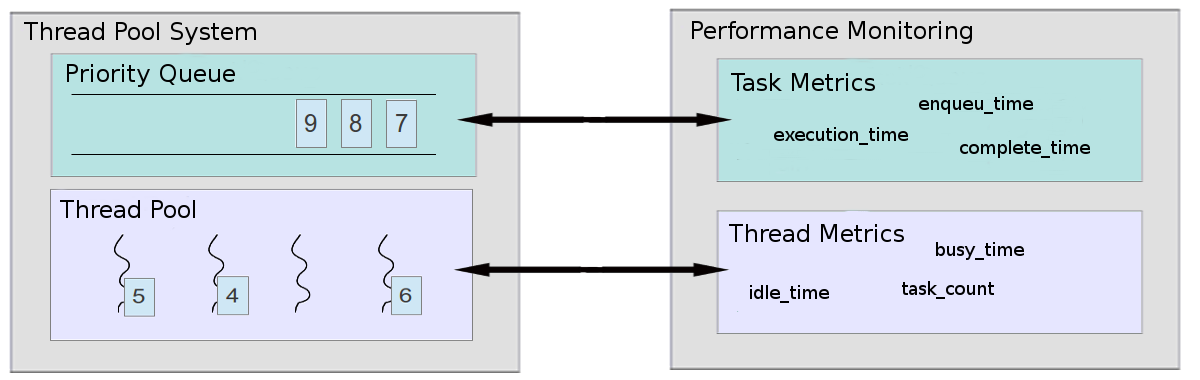
\includegraphics[width=0.9\textwidth]{img/pool_structure.png}
	\end{center}
	\begin{center}
		Thread Pool System
	\end{center}
\end{frame}

\begin{frame}
	\frametitle{Previously on Thread Pool in GeckoDB/BOLSTER}
	\begin{center}
		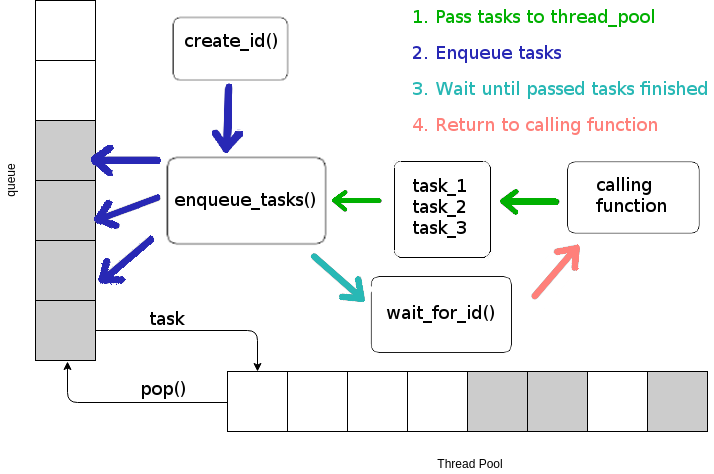
\includegraphics[width=0.8\textwidth]{img/pool_queue.png}
	\end{center}
	\begin{center}
		Enqueuing and Waiting for Tasks
	\end{center}
\end{frame}

\begin{frame}
	\frametitle{Previously on Thread Pool in GeckoDB/BOLSTER}
	\begin{center}
		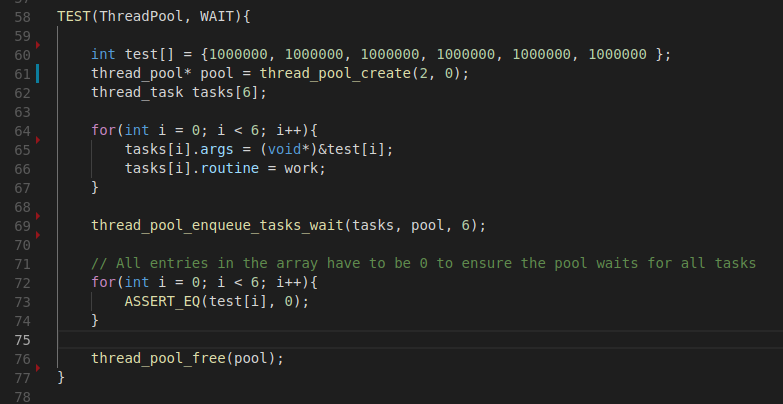
\includegraphics[width=0.9\textwidth]{img/thread_pool_use.png}
		
	\end{center}
	\begin{center}
		Thread Pool Usage
	\end{center}
\end{frame}

\section{Evaluation}
\begin{frame}
	\begin{center}
		\huge Evaluation
	\end{center}
\end{frame}

\begin{frame}
	\frametitle{Evaluation Setup}
	\begin{itemize}
		\item Tests run on different environments, including Windows 10, MacOS Sierra and Archlinux
		\item Presentation results measured on Archlinux with kernel 4.17.2-1 and 24 GB DDR4-SODIMM
		\item Each measure was repeated 3 times and an average value is used
	\end{itemize}
\end{frame}

\begin{frame}
	\frametitle{Evaluation Benchmarks}
	\begin{itemize}
		\item Compare against approximated implementation of BOLSTER (baseline)
		\item Evaluation of waiting time for different thread pool sizes
		\item Utilization of different slot distribution strategies
		\item Utilization of lock-free vs mutex based heap
	\end{itemize}
\end{frame}

\begin{frame}
	\frametitle{Comparison against Baseline Implementation}
	\begin{center}
		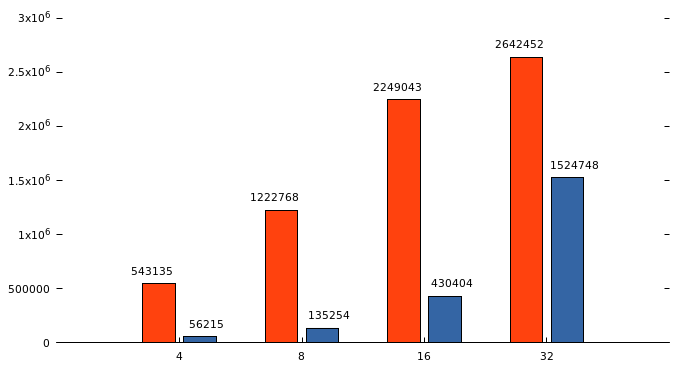
\includegraphics[width=0.8\textwidth]{img/pool_baseline.png}
	\end{center}
	
\end{frame}

\begin{frame}
	\frametitle{Waiting Time Evaluation}
	\begin{center}
		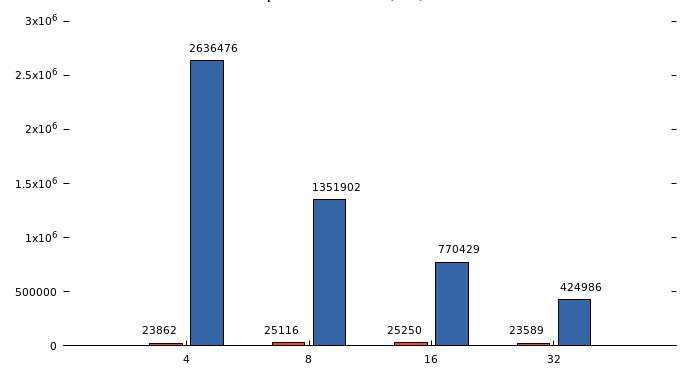
\includegraphics[width=0.8\textwidth]{img/pool_avg.png}
	\end{center}

\end{frame}

\begin{frame}
	\frametitle{Utilization of different slot distribution strategies}
	\begin{center}
		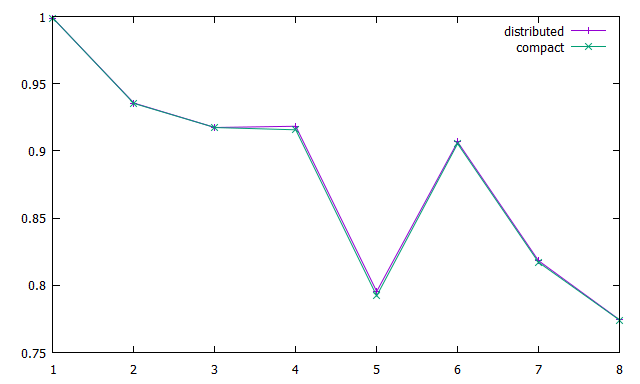
\includegraphics[width=0.8\textwidth]{img/slot_distr.png}
	\end{center}
	\begin{tabular}{c|c|c}
		\#Threads & distributed & compact \\
		1 & 0.998724 & 0.998787 \\
		2 & 0.935569 & 0.935331 \\
		3 & 0.917452 & 0.917384 \\
		4 & 0.918376 & 0.915736 \\
		5 & 0.795493 & 0.792239 \\
		6 & 0.906671 & 0.905388 \\
		7 & 0.818336 & 0.817147 \\
		8 & 0.774444 & 0.77419		
	\end{tabular}
\end{frame}

\begin{frame}
	\frametitle{Utilization of lock-free vs mutex based priority queue}
	\begin{center}
		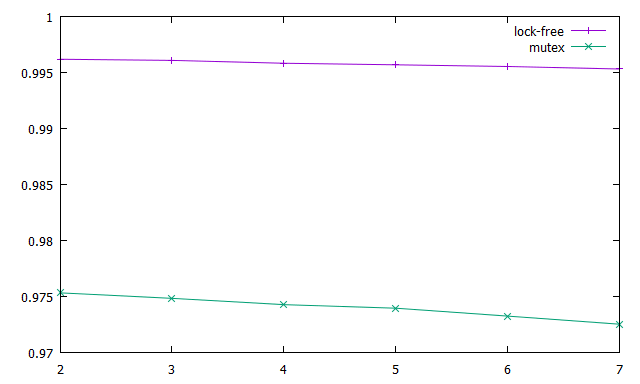
\includegraphics[width=0.8\textwidth]{img/lock_free.png}
	\end{center}
\end{frame}

\section{Summary}
\begin{frame}
	\begin{center}
		\huge Summary
	\end{center}
\end{frame}

\begin{frame}
	\frametitle{Summary}
	\begin{itemize}
		\item Better execution performance as baseline implementation
		\item Constant average waiting time over different pool sizes
		\item Small performance costs for enqueueing and waiting
	\end{itemize}
\end{frame}

\section{Conclusion}
	\begin{frame}
	\begin{center}
		\huge Conclusion
	\end{center}
\end{frame}



\begin{frame}
    \frametitle{Thank you for your attention!}
 	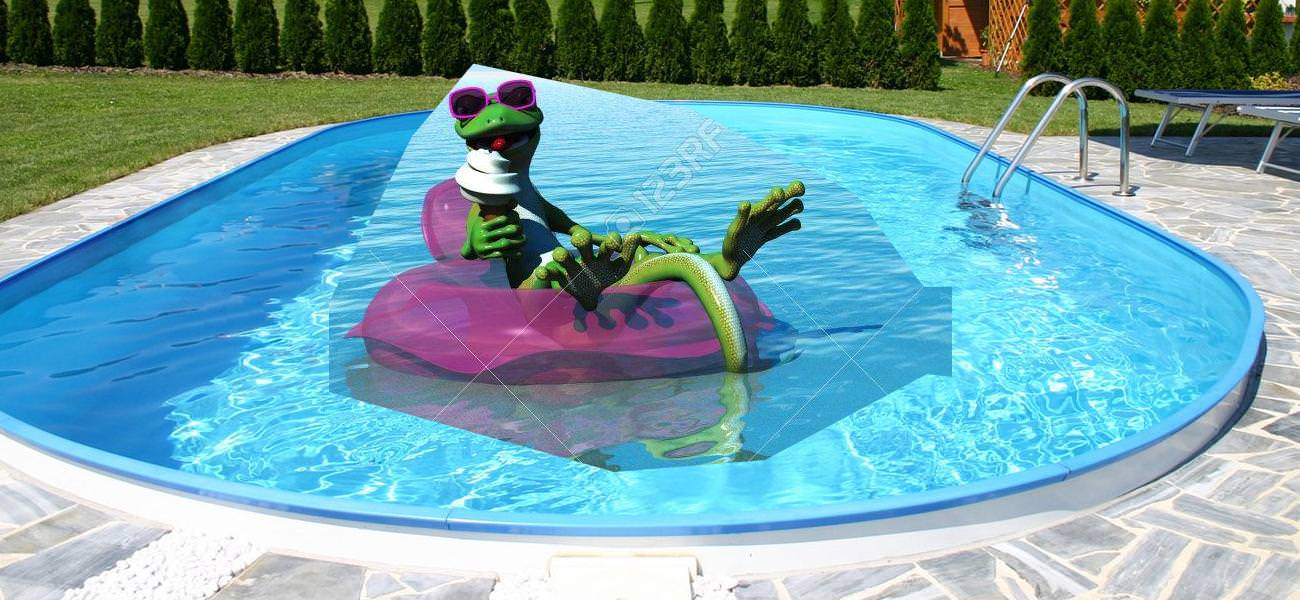
\includegraphics[width=\textwidth]{img/important.jpg}
\end{frame}

\end{document}
